\section{Stability of a Rocket}
\graphicspath{{figures/"Preanalysis&Requirement"/RocketStability/}}
A rocket in order to fly straight has to be stable \cite{web:rocketnasa}. Figure \vref{fig:unstableRocketTrajectory} gives a good example of chaotic trajectory due to unstable design.

\begin{figure} [htbp]
	\centering
	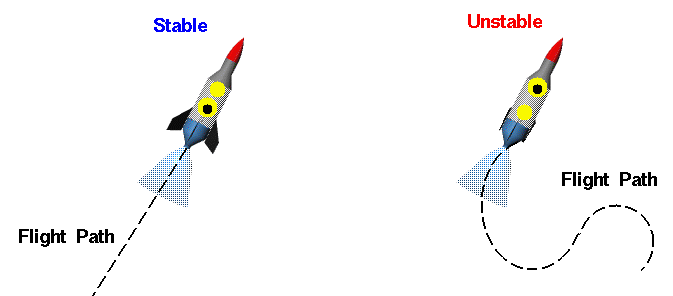
\includegraphics[width=1\linewidth]{UnstableRocketTrajectory}
	\caption{Example of trajectory for an unstable rocket \cite{web:rocketnasa}.}
	\label{fig:unstableRocketTrajectory}
\end{figure}

\subsection{Factors of instability}
To see how a stable rocket has to be designed an analysis of the force applying to the rocket needs to be done. Figure \vref{fig:RocketForceSummary} shows the different situations a rocket encounters during its flight and describes the forces applied in these cases.

\begin{figure} [htbp]
	\centering
	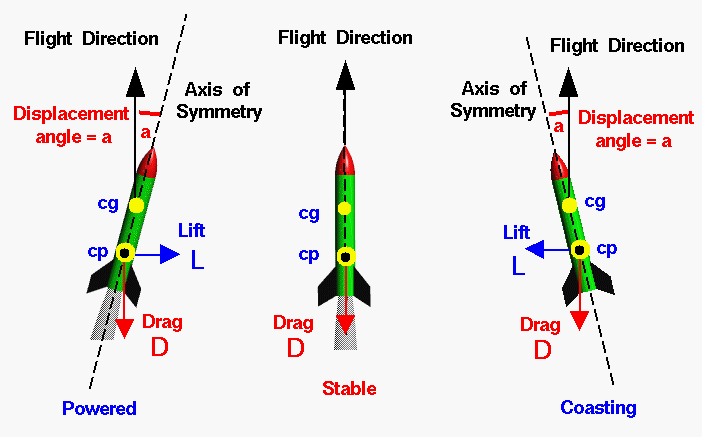
\includegraphics[width=1\linewidth]{ForceSummaryRocket}
	\caption{Summary of forces applied to a rocket during its flight \cite{web:rocketnasa}.}
	\label{fig:RocketForceSummary}
\end{figure}

In figure \vref{fig:RocketForceSummary} two points can be seen on the rockets. The first one CP Center of Pressure is where the  lift and the drag force apply \cite{web:rocketnasa}. The second one is CG Center of Gravity, it is the point where the rocket rotate \cite{web:rocketnasa}. Due to this characteristics the torque applied by the lift and the drag is dependent of the relative positioning between the CG and the CP. Since a rocket tilts due to a torque applied by external forces such as the wind, the lift and the drag has to be oriented so it counters these forces. In order to do so the CP has to be above the CG \cite{web:rocketnasa}.
This means depending of the position of the CP compared to the CG the rocket flight will be either stable or unstable. That is why in simple rocket without any control system the design is done so that CP is indeed above CG.

\subsection{Attitude controller}
The previous design method does not provide a perfectly stable attitude control. To have such precise an active control system is necessary. Full scale rockets use the thrusting force to achieve such control. In order to do so most of them operate with the gimbaled thrust method. It consists of orienting the engine's nozzle and so orienting the thrusting force in the same direction \cite{web:rocketnasa}. However Space X introduces a new propulsion method by using multiple small engines instead of a big one. With this method the thrusting force direction can be controlled by the output of each engine. For smaller rockets orientable fins are used. By changing the orientations of the fins the drag and the lift is changed and so is the attitude of the rocket.